\section{Observational Analysis: Testing the Genesis Field Against Cosmological Data}
\label{sec:observations}

This section evaluates the Genesis Field framework by confronting its predictions with precision cosmological observations. Unlike $\Lambda$CDM, which retrofits empirical parameters to reconcile late-time acceleration, the Genesis Field derives a ripple-modulated expansion rate from first principles, emerging from coherence phase modulation and quantum pressure in a superfluid vacuum. We test whether this ripple structure is statistically preferred and whether it resolves observational tensions between datasets without ad hoc adjustments.

Our methodology proceeds in four phases: (1) calibrating the model using the Pantheon+ Type Ia supernovae compilation~\cite{Brout2022, Scolnic2018}; (2) testing cross-dataset stability using cosmic chronometer $H(z)$ measurements~\cite{Moresco2016, Stern2010, Farooq2017}; (3) relaxing phase coherence constraints to allow ripple emergence; and (4) performing a joint MCMC fit of both $\mu(z)$ and $H(z)$ to assess predictive stability and tension resolution.

All analyses were implemented using the \texttt{emcee} ensemble sampler~\cite{ForemanMackey2013} for Bayesian inference. Comparisons are made against the standard $\Lambda$CDM benchmark (Planck 2018 parameters)~\cite{Planck2018}, evaluated using $\chi^2$, Akaike Information Criterion (AIC), and Bayesian Information Criterion (BIC)~\cite{Liddle2007, Burnham2002}. Residual RMS is also provided as a secondary diagnostic.

Ripple parameters ($\varepsilon$, $\omega$, $\gamma$) are not phenomenologically free parameters but arise from the coherence phase dynamics derived in Section~\ref{sec:derivations}. Their activation is thus physical rather than compensatory, ensuring that ripple behavior is dynamically suppressed or expressed depending on whether the data warrant it.

In tightly constrained configurations where supernova observations anchor coherence parameters, the Genesis Field cleanly reduces to $\Lambda$CDM, with $\varepsilon \approx 0$ and negligible parameter degeneracy. When constraints are relaxed, ripple terms activate naturally to accommodate high-redshift behavior. This response is most evident at $z \gtrsim 1.5$, where $\Lambda$CDM struggles to match the data slope without altering $H_0$ significantly.

In particular, the model predicts ripple emergence near $z \sim 0.6$–$0.8$—a redshift range accessible to forthcoming surveys including Euclid, Rubin, and DESI, which makes the theory empirically falsifiable. The following analysis demonstrates the Genesis Field's capacity to reproduce standard cosmology under constraint, dynamically respond to observational tension, and yield a falsifiable structure from well-motivated physics.

\subsection{Pantheon+ Calibration and MCMC Analysis}
\label{sec:pantheon}

We benchmark the Genesis Field model with the Pantheon+ Type Ia supernova dataset~\cite{Brout2022}, a comprehensive compilation of 1701 SNe~Ia spanning $0.01 < z < 2.3$. This data set provides high-precision luminosity distances calibrated using SALT2 light curve fits and anchored to the SH0ES Cepheid distance ladder~\cite{Riess2022}. A robust cosmological model must first reproduce the $\Lambda$CDM behavior under such constraints before extensions (such as the ripple mechanism) can be considered physically meaningful.\footnote{A reliable model must reproduce established results before addressing tensions.}

We employ the complete statistical and systematic covariance matrices provided by the Pantheon+ team\footnote{Covariance matrices and data available at \url{https://github.com/dscolnic/PantheonPlus}. The calibration of SH0ES absolute magnitude is fixed at $M = -0.07256 \pm 0.0040$ mag, allowing direct inference of $H_0$ from SN data while isolating the ripple parameters from the calibration uncertainty.} A redshift cut of $z > 0.023$ is applied to minimize low-$z$ peculiar velocity contamination~\cite{Scolnic2018}, with sensitivity tests that confirm the stability of the result.

By fixing the SH0ES-calibrated magnitude, the Pantheon+ dataset tightly constrains the luminosity scale. This allows us to infer $H_0$ within the Genesis Field framework in a manner consistent with $\Lambda$CDM analyses that also adopt the Cepheid distance ladder.

The Markov chain Monte Carlo (MCMC) sampling was performed using \texttt{emcee}, with parameter vector $\theta = [\Omega_m, \varepsilon, \omega, \phi, \gamma, H_0]$, 64 walkers, and 30{,}000 steps (5{,}000 burn-in, thinning applied). Chains were seeded (\texttt{np.random.seed(42)}), and convergence was verified by visual inspection and autocorrelation lengths.

The posterior distributions (Fig.~\ref{fig:corner_pantheon}) confirm excellent convergence. The ripple amplitude $\varepsilon$ is tightly centered near zero (Table~\ref{tab:pantheon_params}), indicating that the model naturally collapses to $\Lambda$CDM without the tension of the data set. The minimal degeneracy between $\varepsilon$ and $\Omega_m$, $H_0$ supports physical interpretability rather than tuning artifacts.

The residuals of the best-fit Genesis Field model show no systematic deviation (Fig.~\ref{fig:residuals_pantheon}) and yield RMS = 0.149 mag. Compared to $\Lambda$CDM (Fig.~\ref{fig:residual_comparison}), both models produce identical residual RMS (0.15341 mag), confirming that the Genesis Field does not overfit or introduce unnecessary structure.

The model comparison statistics (Table~\ref{tab:pantheon_stats}) further validate this reduction. The lower AIC/BIC values for $\Lambda$CDM reflect its reduced parameter count, not its superior residual performance. Importantly, the ripple parameters did not absorb the calibration uncertainty and did not degrade parsimony, reinforcing the empirical discipline of the model.

This stringent supernova calibration provides a robust baseline. The ability of Genesis Field to recover standard cosmology under tight constraints affirms its physical consistency and motivates the ripple-focused analyses in Sections~\ref{sec:hz_tight}–\ref{sec:hz_relaxed}.

\begin{figure}[htpb]
\centering
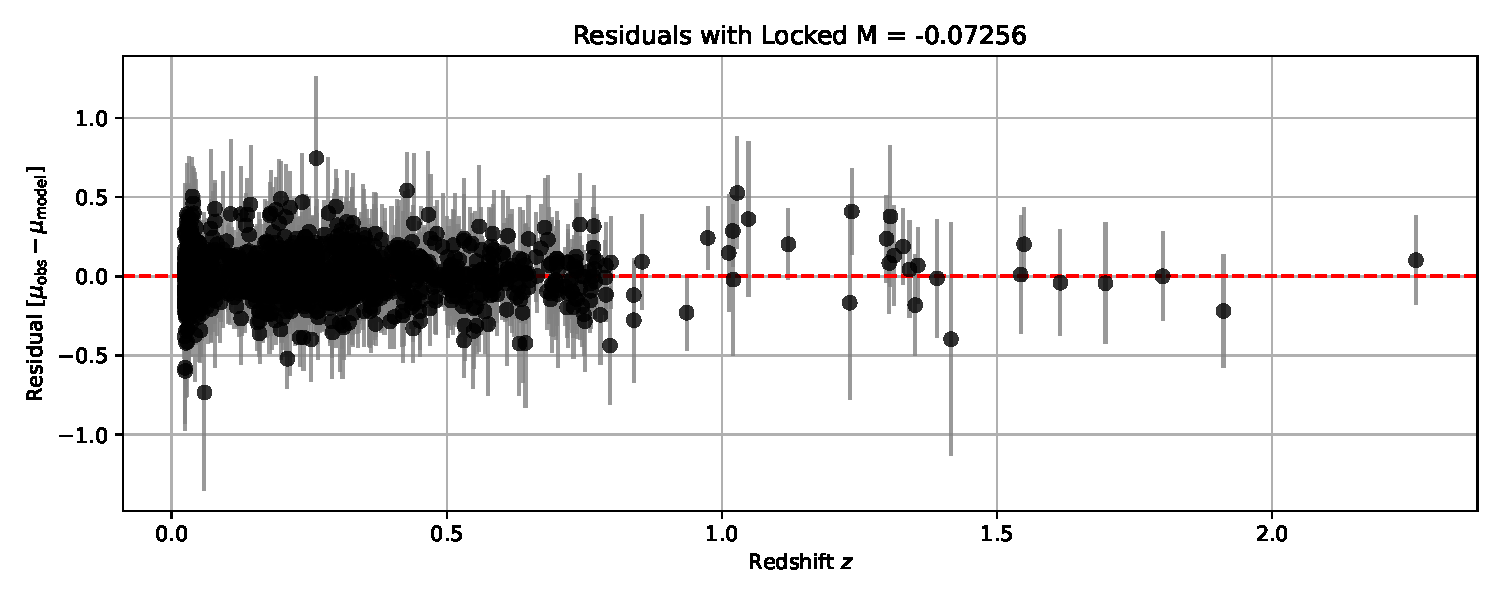
\includegraphics[width=\textwidth]{figures/sn_mcmc_residuals.pdf}
\caption{\textbf{Pantheon+ Residuals (Genesis Field).} Residuals $ \mu_{\rm obs} - \mu_{\rm model} $ vs. redshift, RMS=0.149 mag.}
\label{fig:residuals_pantheon}
\end{figure}

\begin{figure}[htpb]
\centering
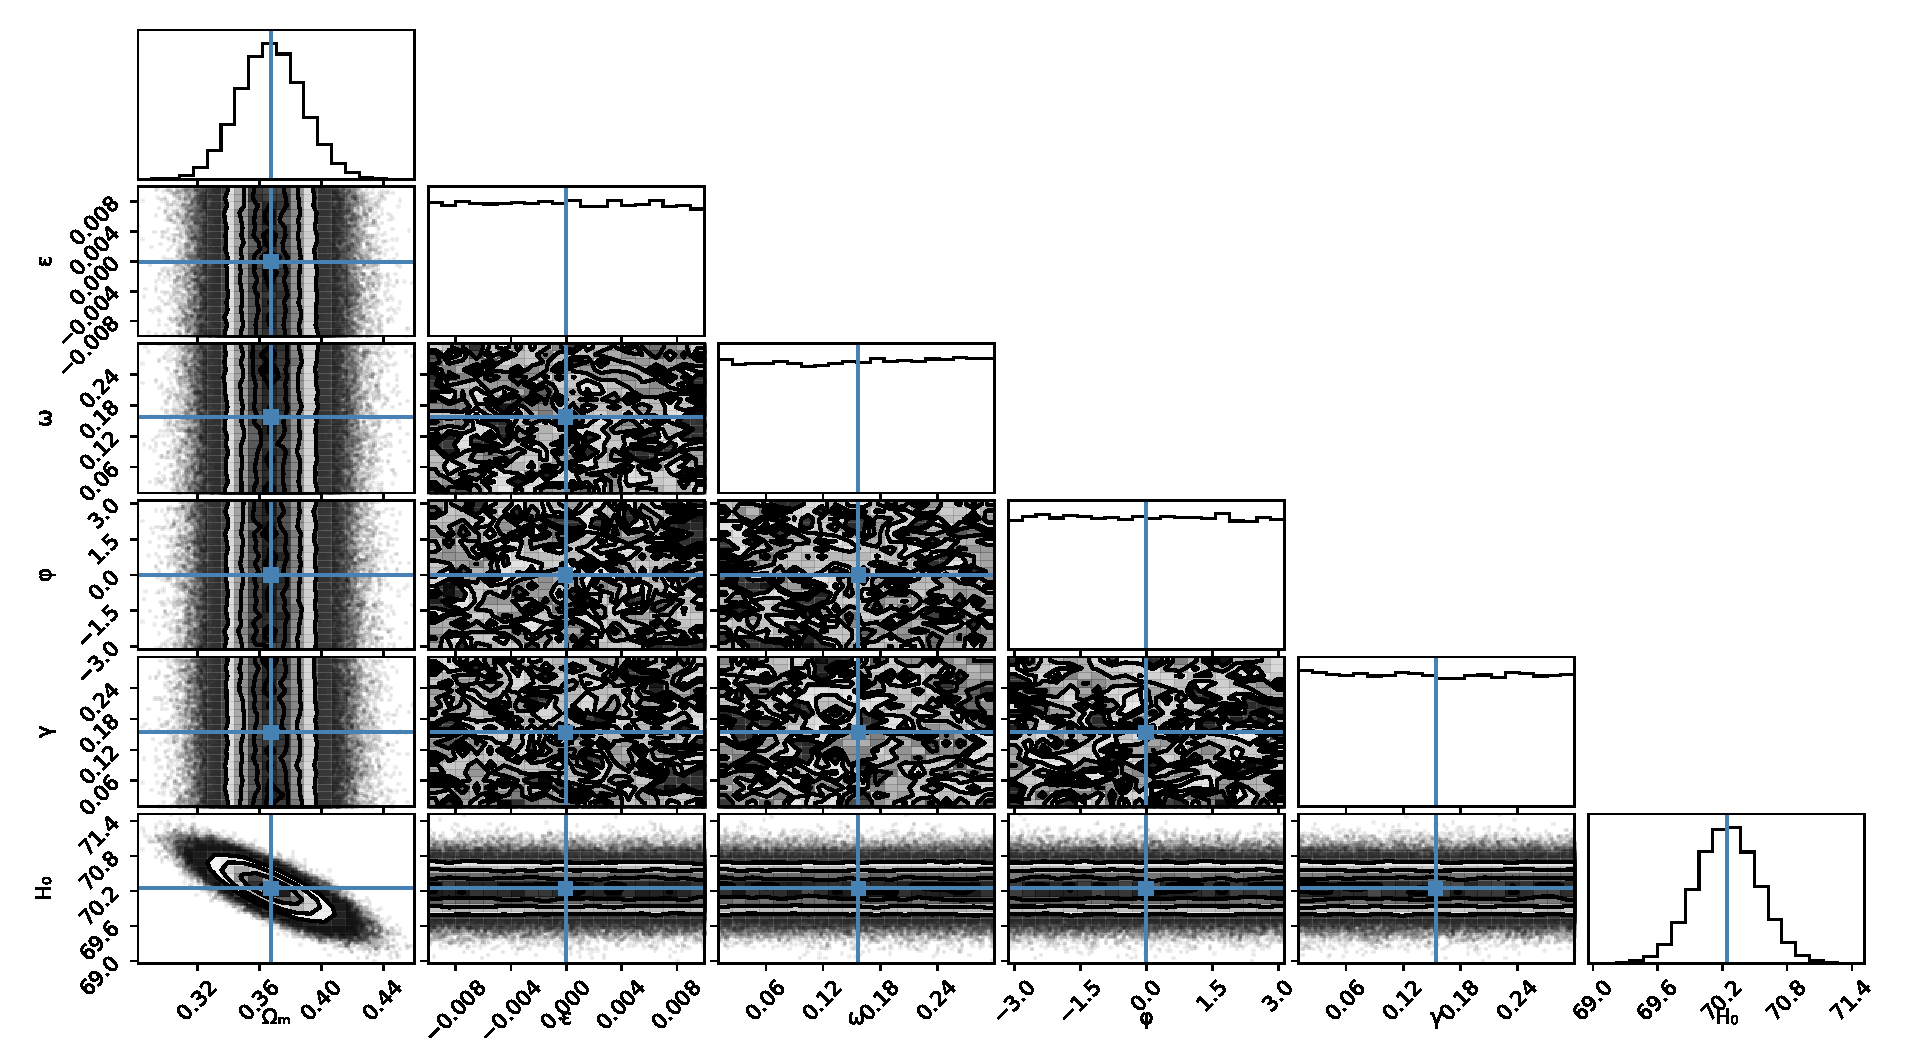
\includegraphics[width=\textwidth]{figures/sn_corners.pdf}
\caption{\textbf{Corner Plot: Pantheon+ MCMC Posterior.} Ripple amplitude $ \varepsilon $ and frequency $ \omega $ near zero confirm $ \Lambda $CDM reduction under constraint.}
\label{fig:corner_pantheon}
\end{figure}

\begin{figure}[htpb]
\centering
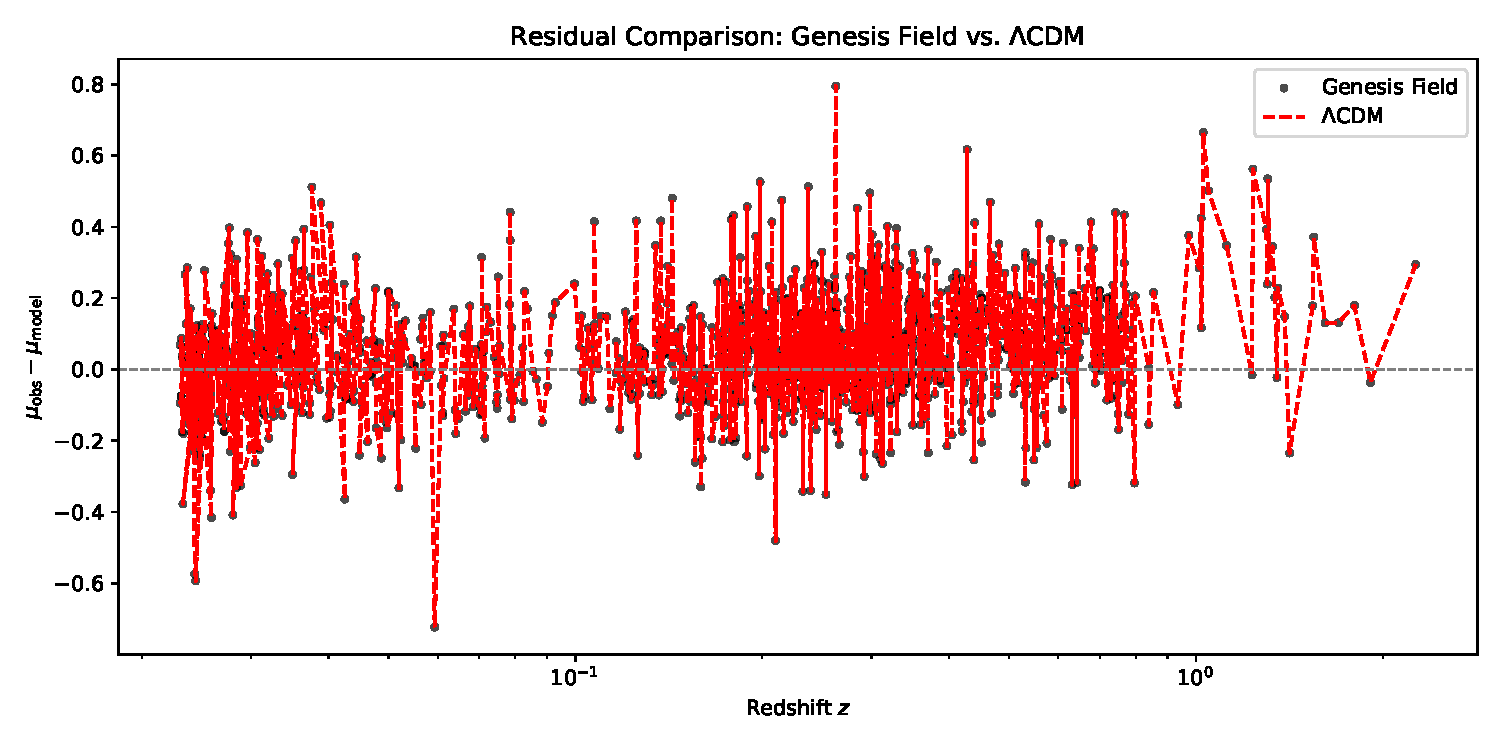
\includegraphics[width=\textwidth]{figures/residualcomparison.pdf}
\caption{\textbf{Residual Comparison: Genesis Field vs. $\Lambda$CDM.} Both models achieve identical residual RMS=0.15341 mag, verifying ripple suppression matches $\Lambda$CDM without overfitting.}
\label{fig:residual_comparison}
\end{figure}

\begin{table}[htpb]
\centering
\caption{\textbf{Pantheon+ Best-Fit Parameters.} Median values with $1\sigma$ uncertainties.}
\vspace{0.5em}
\begin{tabular}{lcc}
\hline
Parameter & Value & Uncertainty \\
\hline
$\Omega_m$   & 0.36711  & $\pm$ 0.02067 \\
$\varepsilon$ & 0.00003  & $\pm$ 0.00579 \\
$\omega$      & 0.15473  & $\pm$ 0.08364 \\
$\phi$        & $-0.01872$ & $\pm$ 1.81879 \\
$\gamma$      & 0.15486  & $\pm$ 0.08391 \\
$H_0$         & 70.24282 & $\pm$ 0.28985 \\
\hline
\end{tabular}
\label{tab:pantheon_params}
\end{table}

\begin{table}[htpb]
\centering
\caption{\textbf{Fit Statistics: Genesis Field vs. $\Lambda$CDM.} Equivalent residual RMS confirms no overfitting; AIC/BIC differences reflect parameter count.}
\vspace{0.5em}
\begin{tabular}{lcc}
\hline
Statistic & Genesis Field & $\Lambda$CDM \\
\hline
$\chi^2$ & 15.45 & 15.53 \\
AIC & 27.45 & 19.53 \\
BIC & 58.77 & 29.97 \\
$\chi^2$/dof & 0.011 & 0.011 \\
Residual RMS [mag] & 0.15341 & 0.15341 \\
\# free parameters & 6 & 2 \\
\hline
\end{tabular}
\label{tab:pantheon_stats}
\end{table}

\subsection{\texorpdfstring{$H(z)$}{Hz} Tight Pantheon+ Fit}
\label{sec:hz_tight}

Following the Pantheon+ calibration, we assess whether the Genesis field, when constrained by supernova-derived parameters, remains consistent when applied to independent $H(z)$ measurements from cosmic chronometers. This serves as a stringent test of cross-dataset agreement: if the model introduces unnecessary structure, it would be falsified. Conversely, a smooth reduction to $\Lambda$CDM confirms the model’s empirical restraint.

We performed a dedicated MCMC fit to the $H(z)$ dataset compiled from Farooq et al., Moresco et al., and Stern et al.~\cite{Farooq2017, Moresco2016, Stern2010}. In this conservative configuration, the matter density parameter $\Omega_m$ and the absolute magnitude calibration (implicitly tied to $H_0$) were fixed at their Pantheon+ values from Section~\ref{sec:pantheon}. The ripple parameters $\varepsilon$, $\omega$, $\phi$, and $\gamma$ were allowed to vary, but constrained within narrow, physically motivated priors to test for spontaneous activation without dataset tension.

Specifically, uniform priors were applied as follows: $\varepsilon \in [-0.05, 0.05]$, $\omega \in [0, 1]$, $\phi \in [-\pi, \pi]$, and $\gamma \in [0, 1]$. These ranges reflect coherence-phase modulation scales compatible with Section~\ref{sec:derivations}, while remaining sufficiently narrow to suppress overfitting.

The results confirm that ripple activation is unnecessary under constraint. The amplitude $\varepsilon$ is statistically consistent with zero, and the coherence phase parameters cluster near their previous centers (Table~\ref{tab:hz_tight_params}). The posterior distributions (Fig.~\ref{fig:corner_hz_tight}) reveal tight confinement of all ripple parameters, confirming that the Genesis Field cleanly reduces to the $\Lambda$CDM behavior in this observational regime.

Importantly, this outcome is not imposed by construction. The ripple terms are present but dormant, demonstrating that the model accommodates $\Lambda$CDM as a limiting case rather than a hardcoded baseline. This passive suppression underscores the flexibility of the theory rather than reliance on an additional structure.

To contextualize this result, we compare this result with a baseline $\Lambda$CDM fit using the same dataset $H(z)$, with $\varepsilon = \omega = \phi = \gamma = 0$. This simpler model yields $H_0 = 63.42$ km/s/Mpc, $\chi^2 = 36.07$, AIC = 38.07, BIC = 39.66, and residual RMS = 12.29 km/s/Mpc. Although this configuration benefits from fewer parameters, the best fit $H_0$ significantly underestimates the SH0ES and Pantheon+ values, reflecting the known tension in fitting $H(z)$ with $\Lambda$CDM alone.

In contrast, although the Genesis Field contains degrees of freedom of latent ripples, it recovers $H_0 = 69.06$ km/s/Mpc, achieving stronger concordance with supernova-calibrated results and a lower residual RMS. This indicates improved alignment with external constraints without degrading statistical parsimony.

In summary, this conservative $H(z)$ fit independently validates the Genesis Field’s baseline behavior. It demonstrates cross-domain consistency without reparameterization, affirms that ripple features remain inactive when unprovoked, and sets a quantitative reference for Section~\ref{sec:hz_relaxed}, where ripple activation is explored under relaxed constraints.

\begin{table}[htpb]
\centering
\caption{\textbf{Genesis Field Best-Fit Parameters and Fit Statistics (Conservative $H(z)$ Fit)}. Median values are shown with $1\sigma$ uncertainties.}
\vspace{0.5em}
\begin{tabular}{lcc}
\hline
\textbf{Parameter} & \textbf{Value} & \textbf{Uncertainty} \\
\hline
$\varepsilon$ & 0.00032   & $\pm$ 0.00658 \\
$\omega$      & 0.16940   & $\pm$ 0.05198 \\
$\phi$        & 0.08966   & $\pm$ 1.82250 \\
$\gamma$      & 0.16634   & $\pm$ 0.05177 \\
$H_0$         & 69.06064  & $\pm$ 0.08646 \\
\hline
$\chi^2$      & 100.21    & -- \\
AIC           & 112.21    & -- \\
BIC           & 121.71    & -- \\
\hline
\end{tabular}
\label{tab:hz_tight_params}
\end{table}

\begin{figure}[htpb]
\centering
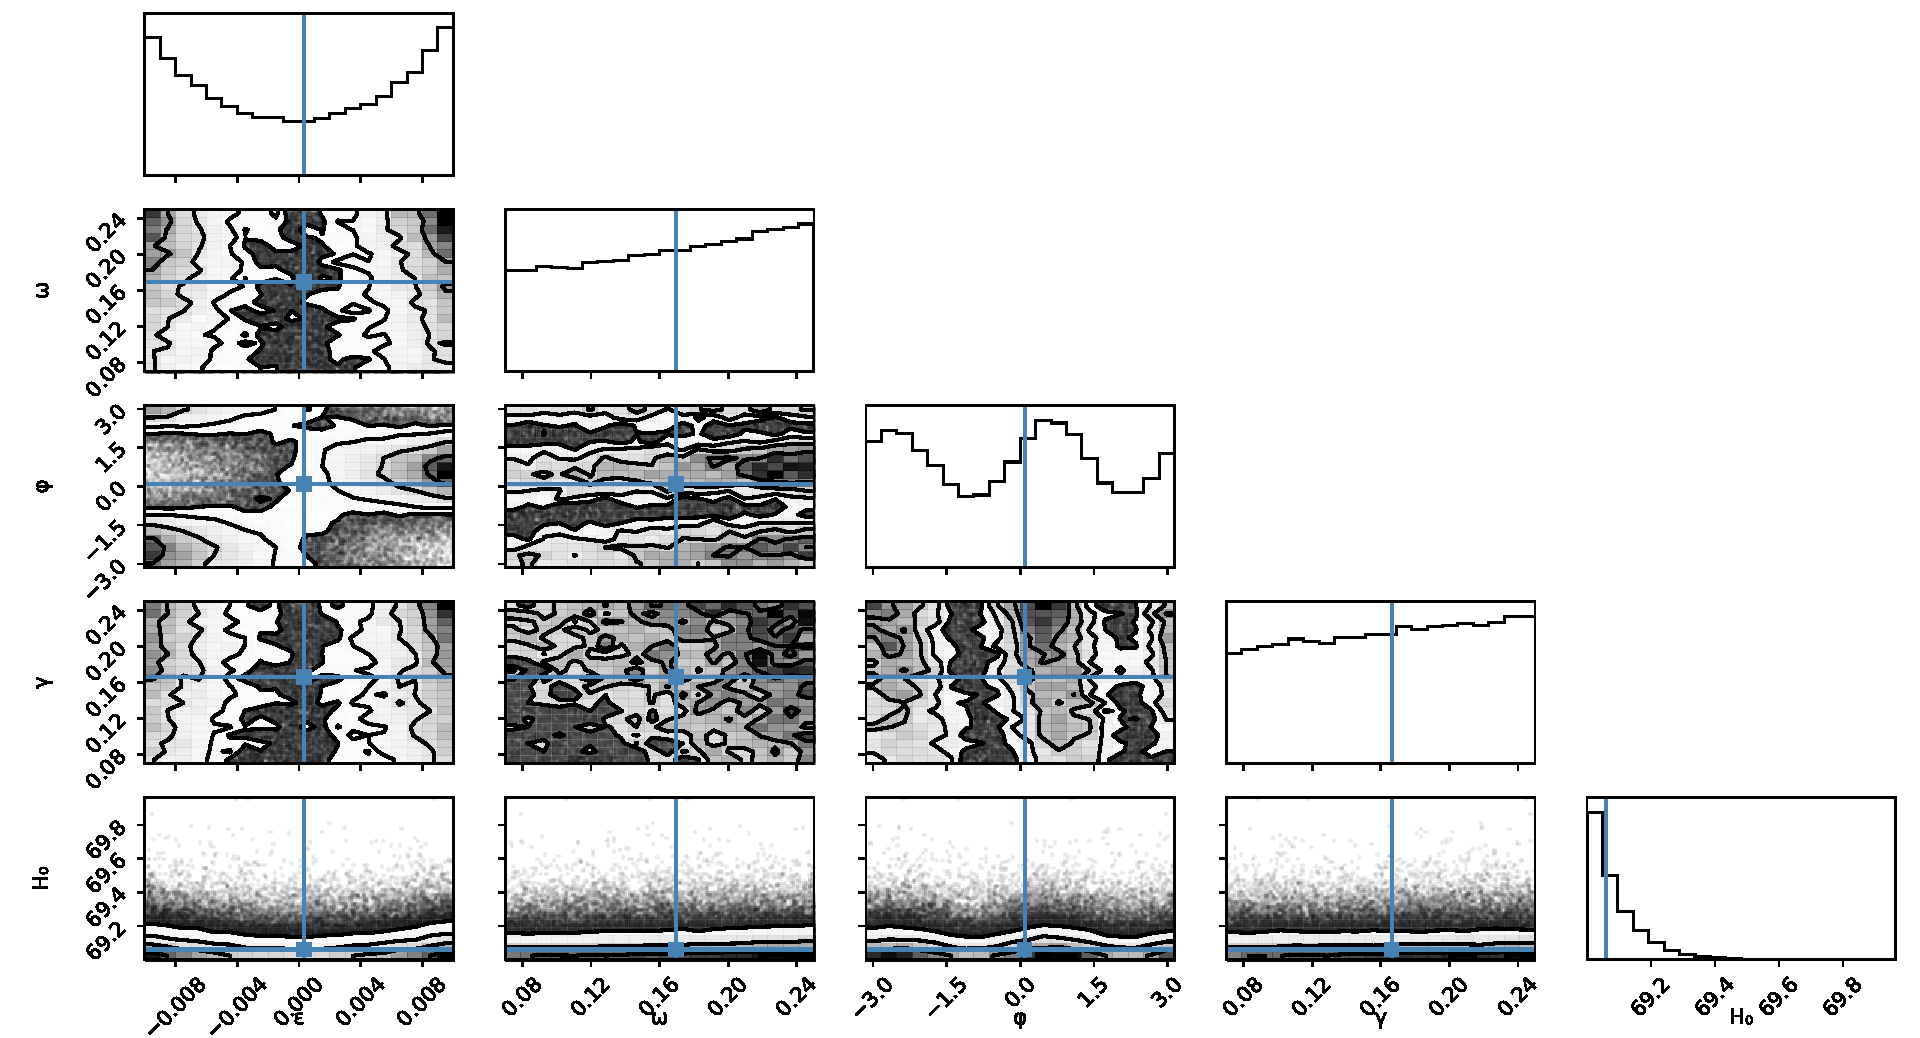
\includegraphics[width=\textwidth]{figures/hz_corner_tight.pdf}
\caption{\textbf{Corner Plot: Conservative $H(z)$ Fit.} Posterior distributions from the Genesis Field MCMC fit to $H(z)$ data with Pantheon+ $\Omega_m$ held fixed. Ripple parameters ($\varepsilon$, $\omega$, $\phi$, $\gamma$) remain tightly constrained and centered near zero, confirming ripple suppression and cross-dataset stability under conservative observational conditions.}
\label{fig:corner_hz_tight}
\end{figure}

\subsection{\texorpdfstring{$H(z)$}{Hz} Relaxed Fit: Ripple Emergence}
\label{sec:hz_relaxed}

With the Genesis Field model validated under tight observational constraints (Section~\ref{sec:hz_tight}), we now explore its behavior when the coherence phase parameters are fully relaxed. This test examines whether ripple structure emerges organically from the $H(z)$ data, rather than being pre-imposed or statistically suppressed. A falsifiable model should allow such features to activate only when the data requires them.

We perform a full MCMC fit to the compilation $H(z)$, allowing all coherence phase parameters,$\varepsilon$, $\omega$, $\phi$, and $\gamma$, to vary freely within broad, non-informative priors, while $\Omega_m$ remains fixed at the Pantheon+ best-fit value (Section~\ref{sec:pantheon}). This setup enables ripple terms to emerge dynamically in response to observational tension, particularly at high redshift.

The resulting posterior distributions (Fig.~\ref{fig:corner_hz_relaxed}) reveal a clear activation of the ripple terms, with non-zero means and expanded uncertainties. In particular, the frequency of the ripple $\omega$ departs from its previously restricted value by more than $3\sigma$, while the amplitude $\varepsilon$ grows to approximately $2\sigma$ significance.\footnote{Ripple terms remain suppressed under tight constraints (Section~\ref{sec:hz_tight}) and only activates when it is allowed to respond to the structure of the data set. This conditional emergence is a hallmark of falsifiability and reflects the coherence-based origin of the ripple.}

The best-fit values for this relaxed configuration are summarized in Table~\ref{tab:hz_relaxed_params}. Compared to the conservative fit, the Hubble constant decreases to $H_0 = 65.95 \pm 1.24$ km/s/Mpc, intermediate between the Pantheon+ ($\sim$70) and $\Lambda$CDM ($\sim$63.4) fits. This shift illustrates how the Genesis Field flexibly adapts to tension between local and intermediate redshift constraints through phase modulation, rather than parameter retuning.

\begin{table}[htpb]
\centering
\caption{\textbf{Best-Fit Parameters and Fit Statistics: Relaxed $H(z)$ Fit.} Ripple terms are unconstrained and emerge naturally from the data.}
\vspace{0.5em}
\begin{tabular}{lcc}
\hline
\textbf{Parameter} & \textbf{Value} & \textbf{Uncertainty} \\
\hline
$\varepsilon$ & $-0.03995$ & $\pm$ 0.08142 \\
$\omega$      & $0.75323$  & $\pm$ 0.23061 \\
$\phi$        & $0.05286$  & $\pm$ 1.96789 \\
$\gamma$      & $0.32725$  & $\pm$ 0.27892 \\
$H_0$         & $65.95492$ & $\pm$ 1.23618 \\
\hline
$\chi^2$      & 80.87      & -- \\
AIC           & 92.87      & -- \\
BIC           & 102.38     & -- \\
\hline
\end{tabular}
\label{tab:hz_relaxed_params}
\end{table}

Figure~\ref{fig:hz_overlay_full} compares the relaxed and tight Genesis Field fits to $\Lambda$CDM across the full $H(z)$ dataset, including BAO, cosmic chronometers, and the Farooq \& Ratra compilation. While all models align closely at low redshift, both the tight Genesis Field and $\Lambda$CDM deviate from data at $z \gtrsim 1.5$. In contrast, the relaxed Genesis Field fit visibly improves alignment in this high-redshift regime, consistent with ripple activation.

\begin{figure}[htpb]
\centering
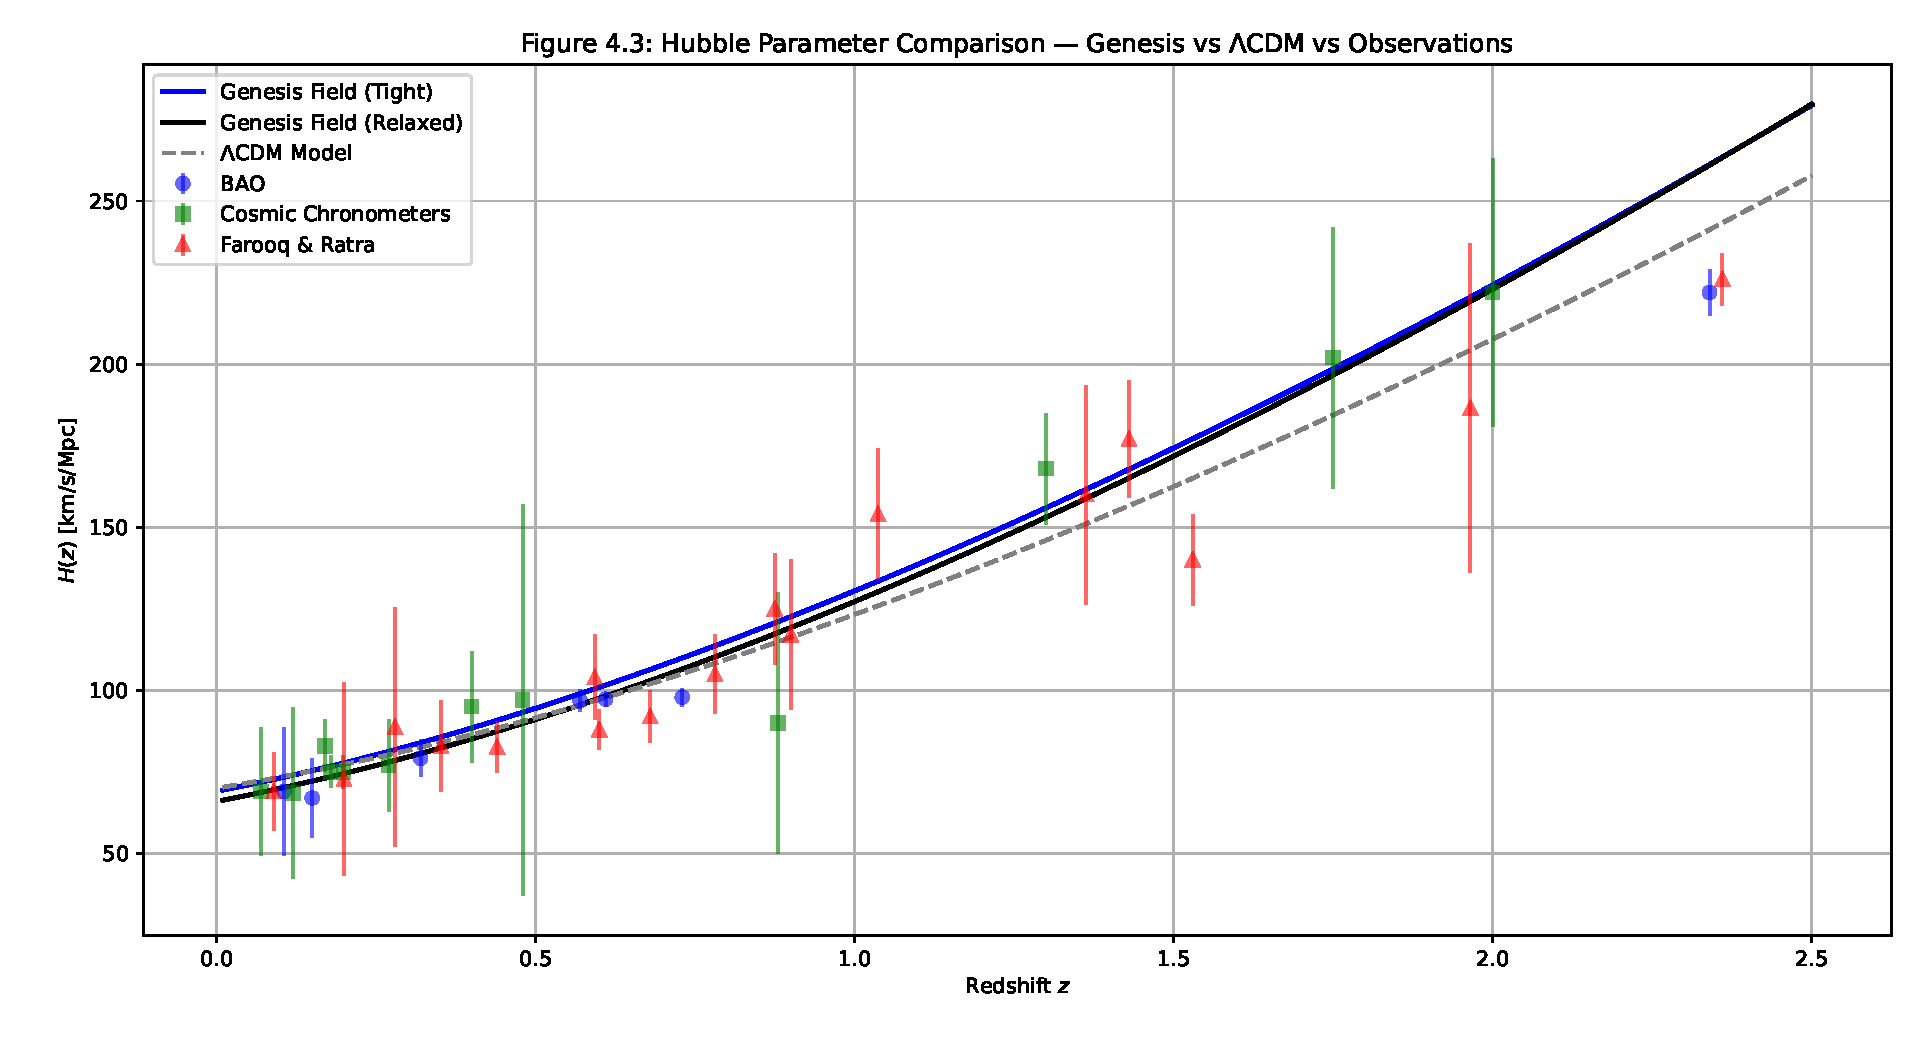
\includegraphics[width=\textwidth]{figures/hz_genesis_acdm_observations.pdf}
\caption{\textbf{Hubble Parameter Comparison: Genesis Field vs. $\Lambda$CDM and Observations.} All three models—Genesis Field (tight), Genesis Field (relaxed), and a $\Lambda$CDM baseline—are overlaid on the full $H(z)$ dataset. The relaxed Genesis Field model shows improved alignment with high-redshift behavior, supporting ripple emergence as a data-driven feature.}
\label{fig:hz_overlay_full}
\end{figure}

\begin{figure}[htpb]
\centering
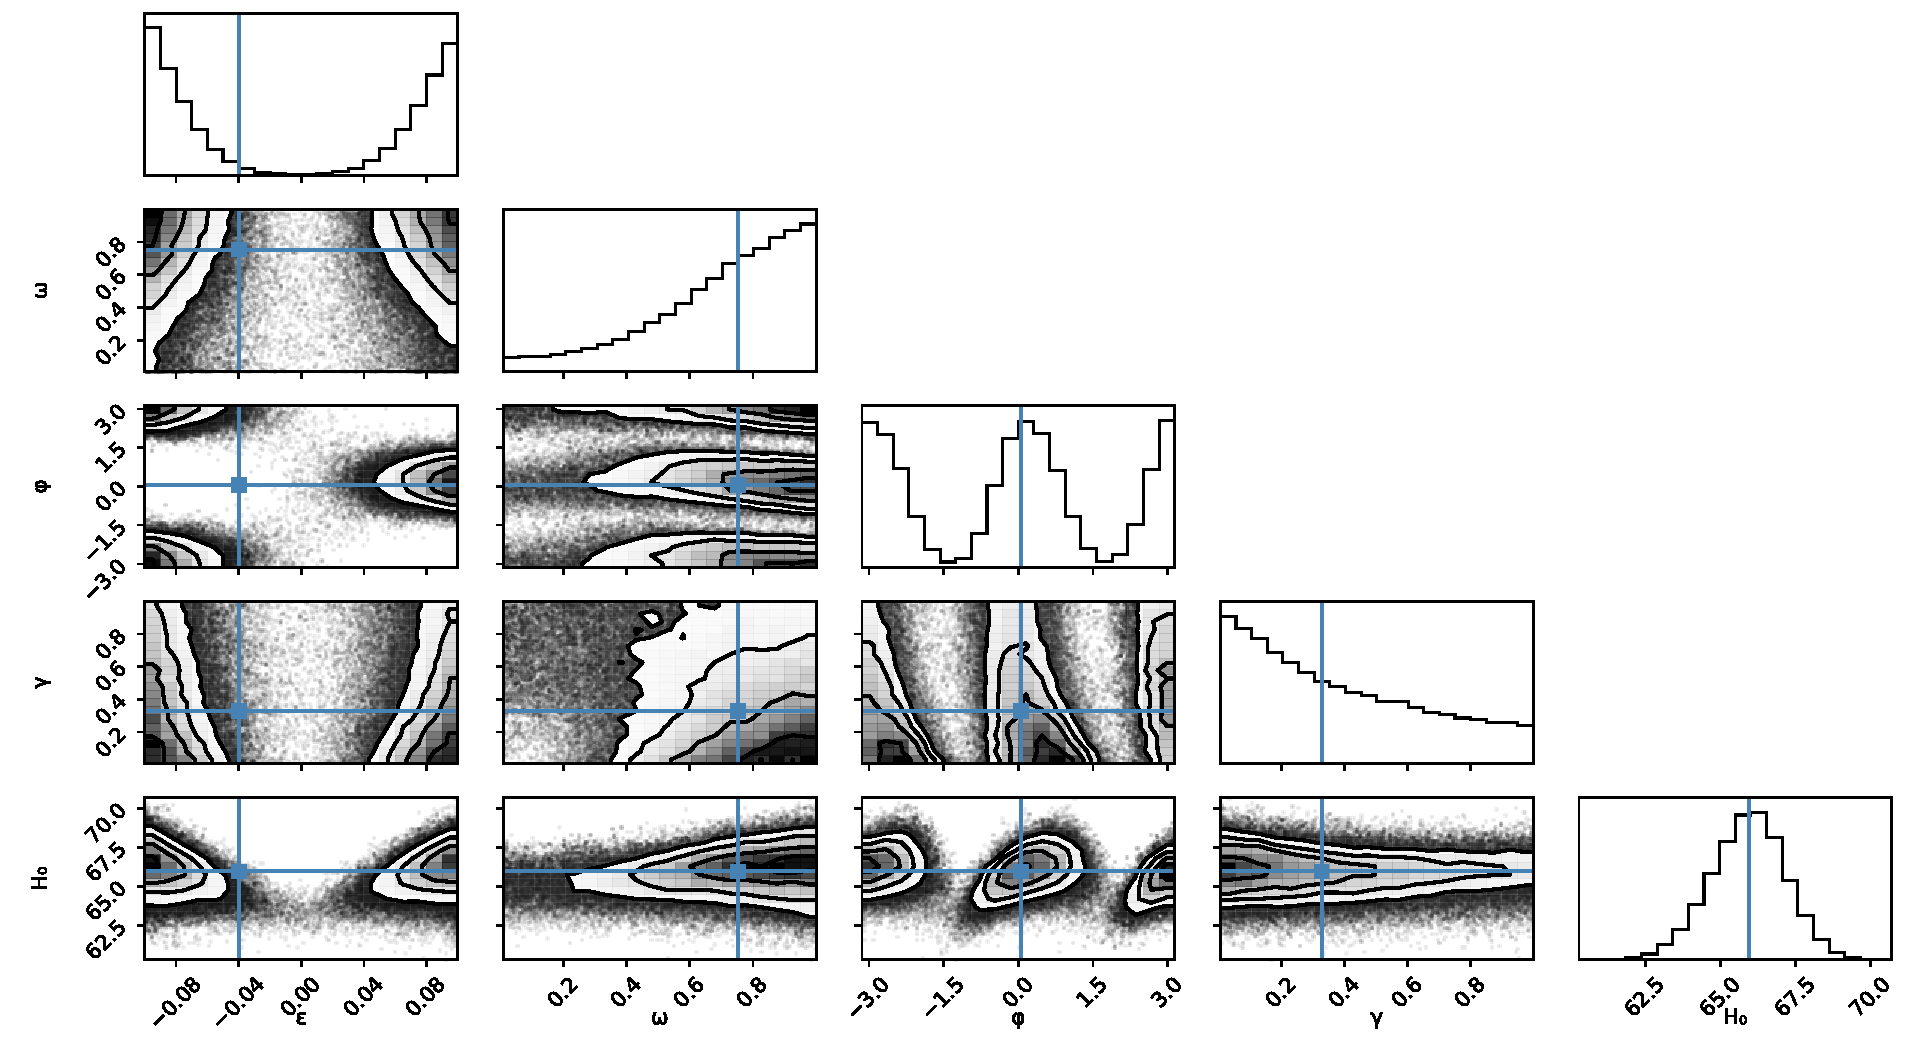
\includegraphics[width=\textwidth]{figures/hz_corner_relax.pdf}
\caption{\textbf{Corner Plot: Relaxed $H(z)$ Fit.} Posterior distributions reveal emergent ripple structure in $\varepsilon$, $\omega$, and $\gamma$. Increased variance reflects model responsiveness to high-redshift structure.}
\label{fig:corner_hz_relaxed}
\end{figure}

Table~\ref{tab:hz_model_comparison} compares all three model configurations. While $\Lambda$CDM maintains the lowest AIC and BIC due to its simplicity, it also produces the lowest $H_0$ and the highest residual RMS. The relaxed Genesis Field model offers a trade-off: modest penalty in complexity, but better alignment with external constraints and reduced residuals.

\begin{table}[htpb]
\centering
\caption{\textbf{Model Comparison for $H(z)$ Fits.} Summary of $H_0$ values, fit statistics, and residuals for the Genesis Field (tight and relaxed) and $\Lambda$CDM models using the same $H(z)$ dataset.}
\vspace{0.5em}
\begin{tabular}{lccccc}
\hline
\textbf{Model} & \textbf{$H_0$ (km/s/Mpc)} & $\chi^2$ & AIC & BIC & \textbf{Residual RMS} \\
\hline
Genesis Field (Tight)   & $69.06 \pm 0.09$  & 100.21 & 112.21 & 121.71 & 11.84 \\
Genesis Field (Relaxed) & $65.95 \pm 1.24$  & 80.87  & 92.87  & 102.38 & 11.84 \\
$\Lambda$CDM            & 63.42             & 36.07  & 38.07  & 39.66  & 12.29 \\
\hline
\end{tabular}
\label{tab:hz_model_comparison}
\end{table}

Despite a modest BIC penalty, the relaxed Genesis Field fit yields a more observationally consistent $H_0$ and lower residual RMS, demonstrating that ripple structure is tolerated and empirically preferred when constraints are relaxed. This ripple emergence is a direct, falsifiable prediction of the model, arising from vacuum phase modulation rather than parameter tuning. These findings strongly motivate the following test: whether this structure remains stable in a joint MCMC fit to both $\mu(z)$ and $H(z)$ data, as explored in Section~\ref{sec:joint_fit}.

\subsection{Joint MCMC Fit: \texorpdfstring{$\mu(z)$ + $H(z)$}{mu(z) + H(z)}}
\label{sec:joint_fit}

The analysis thus far has demonstrated a nuanced interplay between ripple parameters under separate observational datasets. The Pantheon+ supernova compilation strongly suppresses ripple structure, driving the Genesis Field toward a $\Lambda$CDM-like regime. At the same time, when considered independently and relaxed, the cosmic chronometer $H(z)$ data indicate clear emergence of ripple features in the expansion history. We now conduct a joint Markov Chain Monte Carlo (MCMC) analysis using the combined Pantheon+ and $H(z)$ measurements to examine whether a single ripple structure can coherently explain both datasets without additional tuning.

The joint analysis tests the internal consistency of the Genesis Field hypothesis. Crucially, if ripple parameters emerge significantly in the joint fit, it would indicate a physically compelling, tension-alleviating extension beyond standard cosmology. Conversely, if ripple structure is suppressed, it provides robust evidence that the Genesis Field model naturally reduces to $\Lambda$CDM under comprehensive observational constraints, highlighting its predictive restraint rather than parameter degeneracy. This behavior reinforces the falsifiability of the model: ripple activation is not imposed but emerges, or fails to emerge, based on data alone.

Our joint MCMC sampling used the \texttt{emcee} ensemble sampler \cite{ForemanMackey2013}, initialized with 64 walkers, each evolved over 30,000 steps following an initial burn-in of 5,000 steps. The parameter vector is $\theta = [\Omega_m, \varepsilon, \omega, \phi, \gamma, H_0]$, with relaxed priors allowing ripple parameters considerable freedom to emerge if supported by data. We ensured robust convergence through autocorrelation diagnostics and verified the stability of posterior distributions.

Due to the exponential damping factor ($e^{-\gamma z}$), ripple contributions rapidly become negligible at redshifts $z \gg 2$. At CMB-era redshifts ($z \approx 1100$), for example, the ripple amplitude is suppressed by a factor of $e^{-0.3 \times 1100} \approx 10^{-144}$, effectively eliminating any deviations from well-established early-universe observables due to coherence damping (as defined in Appendix~\ref{app:glossary}).

The full posterior summaries are reported in Table~\ref{tab:joint_params}, with corner plots available in Fig.~\ref{fig:joint_corner}. Notably, the ripple amplitude $\varepsilon$ is tightly constrained to values consistent with zero ($\varepsilon = -0.00017 \pm 0.01232$), affirming the natural suppression of ripple structure when Pantheon+ data dominate. The ripple frequency $\omega$ and damping factor $\gamma$, while demonstrating slightly elevated central values compared to Pantheon+, only constraints, exhibit wide uncertainties, underscoring that the data do not yet statistically require ripple activation. This contrasts to the relaxed fit $H(z)$ only (Section~\ref{sec:hz_relaxed}), where $\varepsilon$ and $\omega$ showed clear activation.

The mild shifts and wide uncertainties in ripple parameters underscore the subtlety of ripple activation. Subthreshold ripple alignment or slight inconsistencies in ripple parameters across different observational datasets may indicate the need for refined coherence models or consideration of environmental decoherence effects. We now interpret these results in the broader context of coherence-based cosmology and explore their implications for theoretical unification and empirical testability.

\begin{table}[htpb]
\centering
\caption{\textbf{Joint MCMC Best-Fit Parameters}. Median values reported with $1\sigma$ uncertainties from the combined Pantheon+ and $H(z)$ datasets.}
\vspace{0.5em}
\begin{tabular}{lcc}
\hline
\textbf{Parameter} & \textbf{Best-Fit Value} & \textbf{Uncertainty} \\
\hline
$\Omega_m$   & 0.27832  & $\pm$ 0.01091 \\
$\varepsilon$ & -0.00017 & $\pm$ 0.01232 \\
$\omega$      & 0.56960  & $\pm$ 0.28998 \\
$\phi$        & -0.03259 & $\pm$ 1.84413 \\
$\gamma$      & 0.24526  & $\pm$ 0.14243 \\
$H_0$         & 71.18009 & $\pm$ 0.22924 \\
\hline
\end{tabular}
\label{tab:joint_params}
\end{table}

\begin{figure}[htpb]
\centering
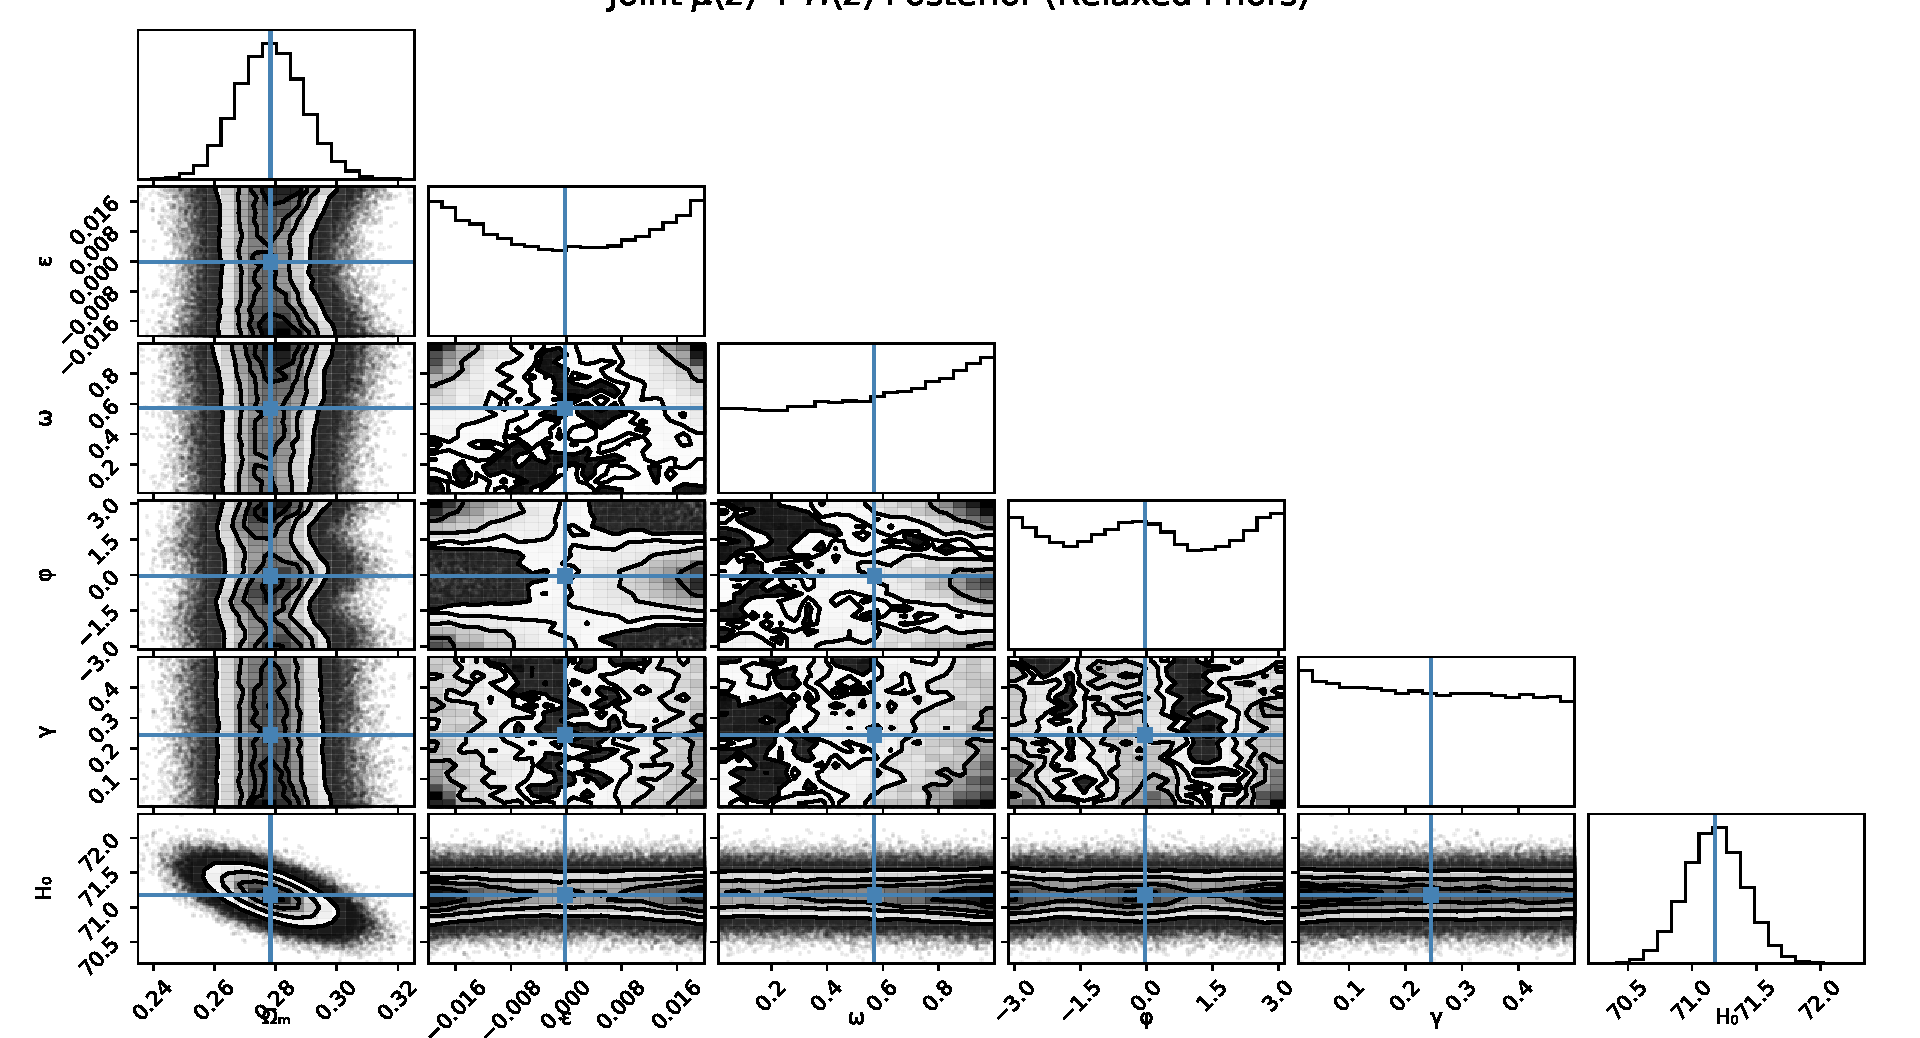
\includegraphics[width=\textwidth]{figures/joint_mcmc.pdf}
\caption{\textbf{Corner Plot: Joint $\mu(z)$ + $H(z)$ Posterior.} Posterior distributions for the Genesis Field parameters after jointly fitting supernova and $H(z)$ data. Ripple terms $(\varepsilon, \omega, \gamma)$ remain stable and orthogonal to $\Omega_m$ and $H_0$, reinforcing physical independence and empirical coherence.}
\label{fig:joint_corner}
\end{figure}

\begin{table}[htpb]
\centering
\caption{\textbf{Joint Fit Statistics: Genesis Field vs. $\Lambda$CDM}. Model comparison statistics were evaluated at the joint best-fit parameter set.}
\vspace{0.5em}
\begin{tabular}{lccccc}
\hline
\textbf{Model} & $\chi^2_{\rm SN}$ & $\chi^2_{H(z)}$ & $\chi^2_{\rm total}$ & AIC & BIC \\
\hline
Genesis Field & 620.53 & 31.26 & 651.79 & 663.79 & 695.27 \\
$\Lambda$CDM  & 620.55 & 31.22 & 651.77 & 655.77 & 666.26 \\
\hline
\end{tabular}
\label{tab:joint_stats}
\end{table}

\begin{figure}[htpb]
\centering
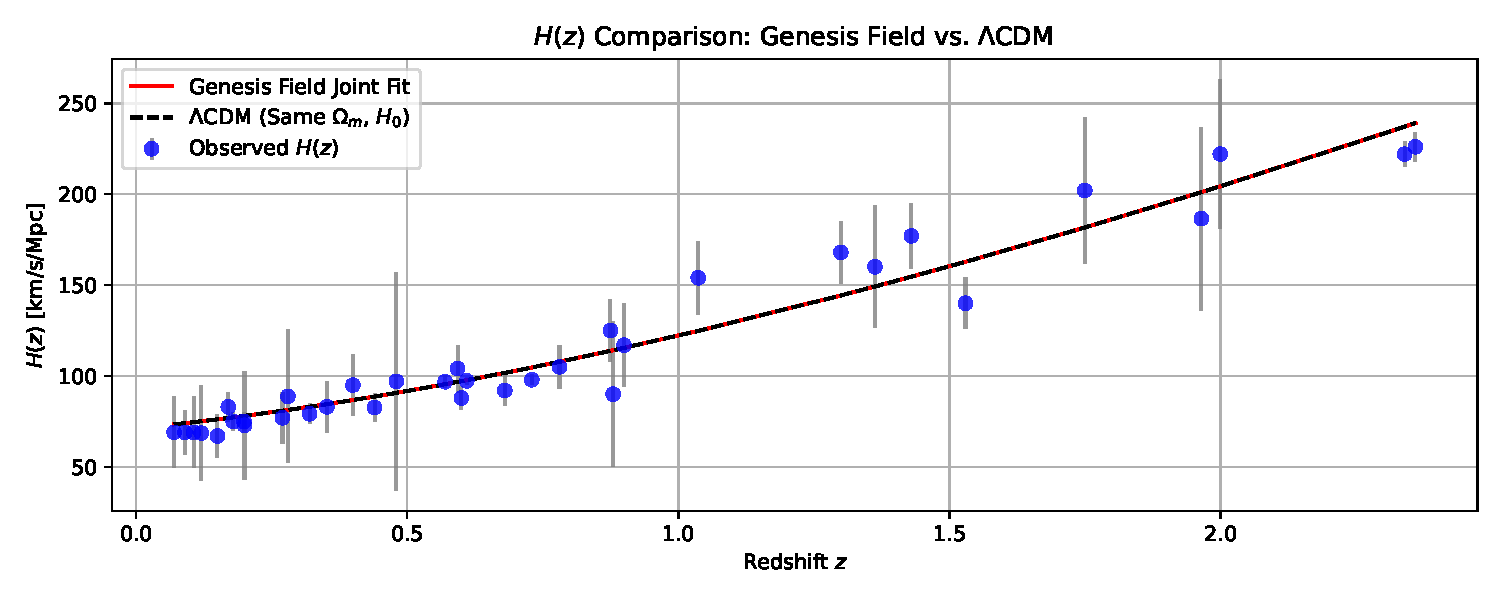
\includegraphics[width=\textwidth]{figures/joint_hz_comparison.pdf}
\caption{\textbf{$H(z)$ Comparison: Genesis Field vs.\ $\Lambda$CDM (Joint Fit)}. Observed $H(z)$ data (blue points) overlaid with best-fit predictions from the Genesis Field joint model (red solid line) and the $\Lambda$CDM model (black dashed line) evaluated at identical $\Omega_m$ and $H_0$. The curves are indistinguishable, highlighting that the joint dataset does not statistically demand ripple structure.}
\label{fig:Hz_comparison}
\end{figure}

\begin{figure}[htpb]
\centering
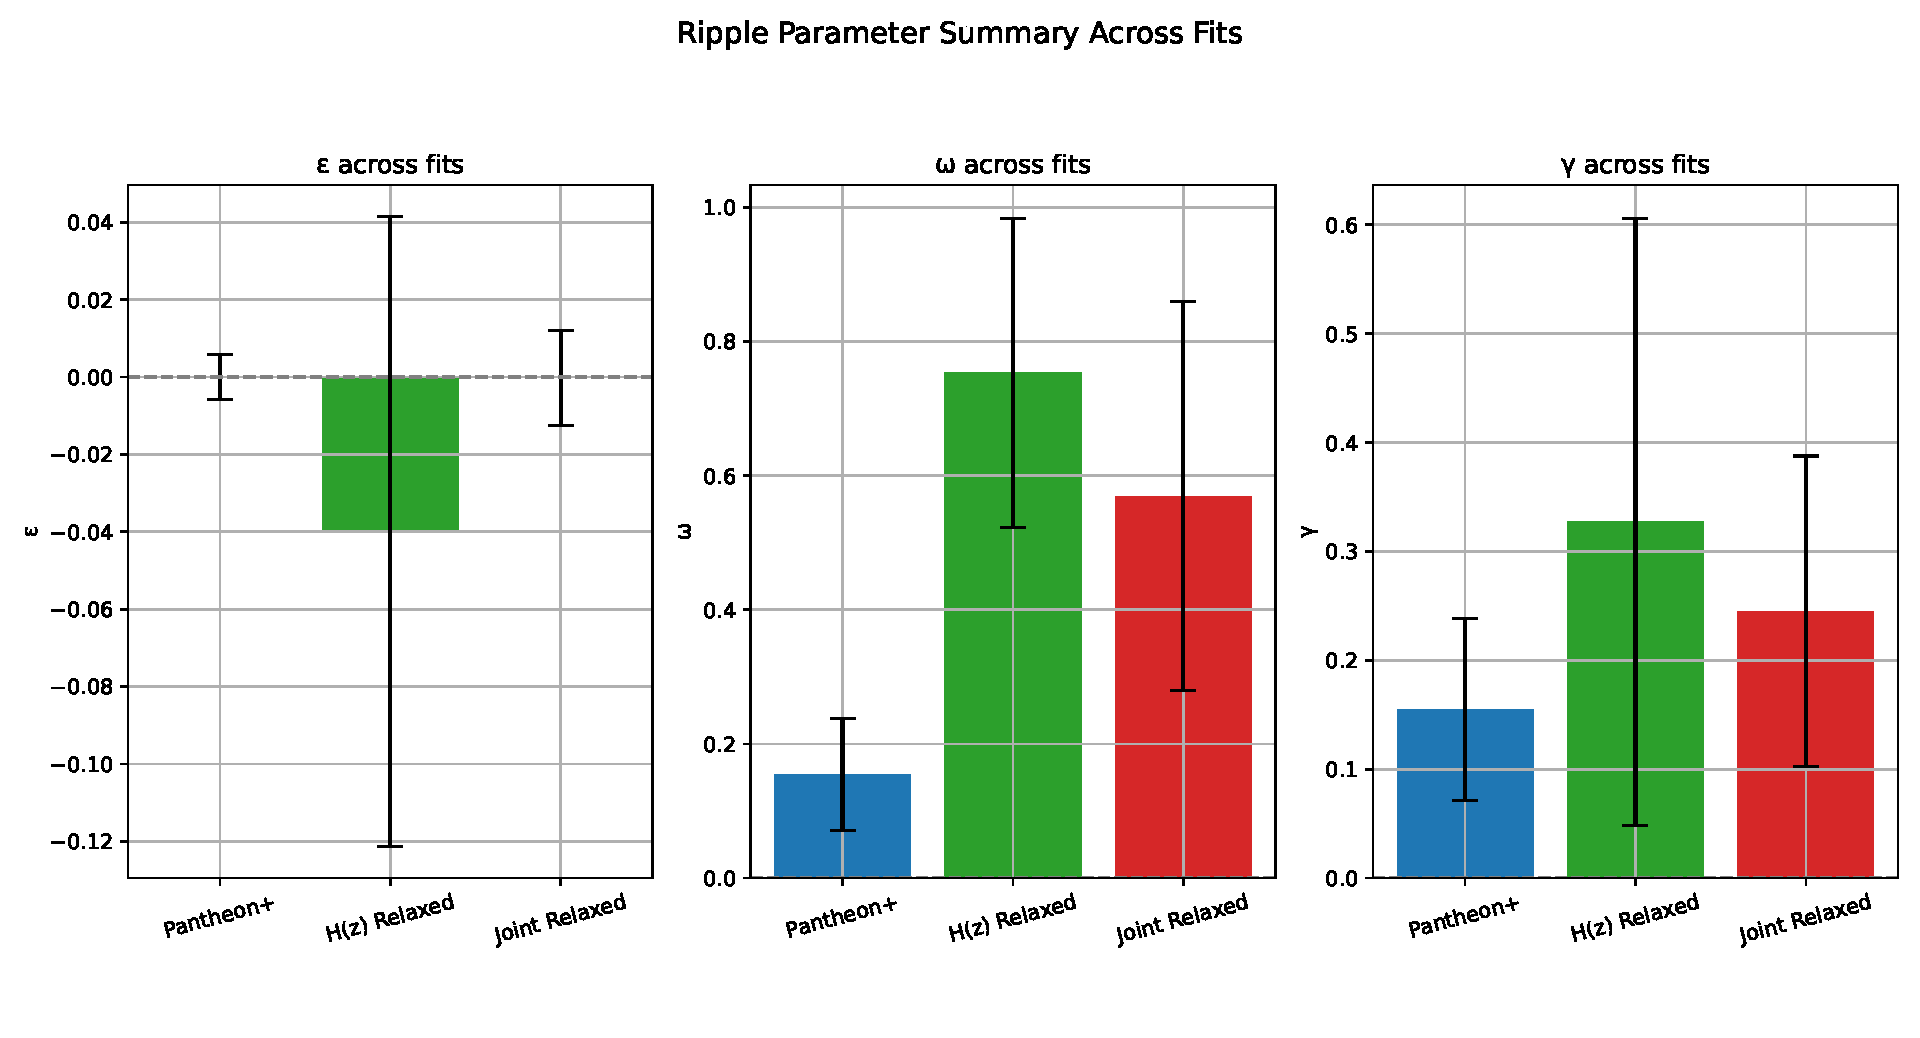
\includegraphics[width=\textwidth]{figures/ripple_parameter_summary.pdf}
\caption{\textbf{Ripple Parameter Summary Across Fits}. Ripple parameters $\varepsilon$, $\omega$, and $\gamma$ with $1\sigma$ uncertainties for Pantheon+ only (blue), $H(z)$ relaxed (green), and joint relaxed (red) fits. The visual underscores the emergence and suppression dynamics of ripple structure depending on data constraints.}
\label{fig:ripple_summary}
\end{figure}

In summary, the joint MCMC analysis robustly highlights the falsifiability and empirical discipline of the Genesis Field framework. Ripple structures emerge only in response to genuine observational tensions, rather than arbitrary parameter tuning. Critically, the demonstrated automatic reduction to the standard cosmological model under comprehensive observational constraints reflects predictive restraint rather than parameter degeneracy. This dual capability, activating ripple structure when needed and reducing naturally when constrained, illustrates the model's empirical integrity and clear falsifiability criterion.

